\section{Auswertung}

In dem folgenden Abschnitt sollen mithilfe der aufgenommenen Daten die Lebensdauer
der Myonen bestimmt werden. Die Fehlerberechnung wird mit dem
Paket $\textit{uncertainties}$ in $\textit{Python}$ durchgeführt. Da die Werte
bei Berechnung des Plateaus sowie Ermittlung der Lebensdauer fehlerbehaftet sind,
wird für die Regression ein gewichteter Fit mit der Funktion \textit{curve\_fit}
durchgeführt.

\subsection{Einstellung der Verzögerungszeit}

Um die abgegebenen Signale der Koinzidenzapparatur zu maximieren, wird während
der Kalibrierung des Versuches die Verzögerungszeit $T\ua{VZ}$ varriert. Die am
Ausgang der Apparatur gemessene Anzahl an Signalen wird in Tabelle \ref{tab:Verzögerung}
wiedergegeben und ist in Abbildung \ref{fig:Plateau} graphisch dargestellt.
In den interessanteren Bereichen wurden mehrere Messwerte genommen, allerdings
ist in Tabelle \ref{tab:Verzögerung} immer nur der gemittelte
Wert eingetragen. Die jeweiligen Zeiten sind mit einem Sternchen markiert. Ein
negatives Vorzeichen bei der Verzögerungszeit entspricht einer Verzögerung bei
dem linken SEV und ein positives Vorzeichen dementsprechend einer Verzägerun
bei dem rechten SEV. Es handelt sich um Anzahlen, deshalb sind die Zahlen auf
natürliche Zahlen gerundet. Als Fehler wird für den Wert $n$ immer $\sqrt{n}$
angenommen.

\begin{figure}
  \centering
  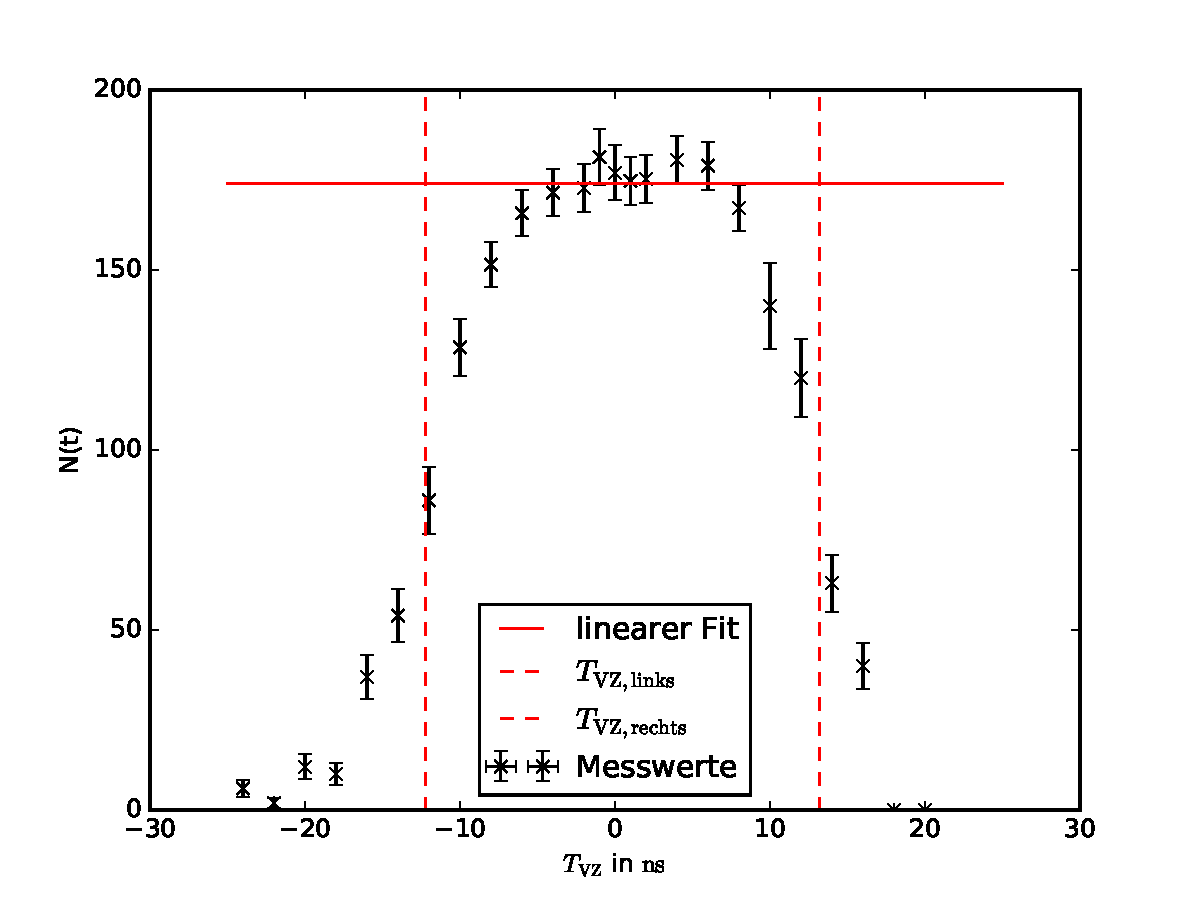
\includegraphics[width = \textwidth]{Pics/Plateau.pdf}
  \caption{Plateau für die Impulsrate bei varrierter Verzögerungszeit.}
  \label{fig:Plateau}
\end{figure}

\begin{table}
  \centering
  \caption{Messwerte bei Einstellung der Verzögerungszeit.}
  \label{tab:Verzögerung}
  \begin{tabular}{c c c c}
    \toprule
    $T\ua{VZ}$ in $\su{ns}$ & $N(T\ua{VZ})$ $\pm$ $\increment N$ &
    $T\ua{VZ}$ in $\su{ns}$ & $N(T\ua{VZ})$ $\pm$ $\increment N$  \\
    \midrule
    -24  &  6  $\pm$ 2  & 0*   & 177 $\pm$ 8  \\
    -22  &  2  $\pm$ 1  & 1*   & 175 $\pm$ 7  \\
    -20  & 12  $\pm$ 3  & 2*   & 176 $\pm$ 7  \\
    -18  & 10  $\pm$ 3  & 4*   & 181 $\pm$ 7  \\
    -16  & 37  $\pm$ 6  &  6*  & 179 $\pm$ 7  \\
    -14  & 54  $\pm$ 7  & 8*   & 168 $\pm$ 6  \\
    -12  & 86  $\pm$ 9  & 10   & 140 $\pm$ 12 \\
    -10* & 129 $\pm$ 8  & 12   & 120 $\pm$ 11 \\
    -8*  & 152 $\pm$ 6  & 14   & 63  $\pm$ 8  \\
    -6*  & 166 $\pm$ 6  & 16   & 40  $\pm$ 6  \\
    -4*  & 172 $\pm$ 7  & 18   &  0  $\pm$ 0  \\
    -2*  & 173 $\pm$ 7  & 20   &  0  $\pm$ 0  \\
    -1*  & 181 $\pm$ 8  &  0   &  0           \\
    \bottomrule
  \end{tabular}
\end{table}

\newpage

\begin{equation}
  N(T\ua{VZ}) = 0\cdot T\ua{VZ} + N\ua{max}
  \label{eqn:FitPlateau}
\end{equation}

Durch die Werte im Intervall $T\ua{VZ} \in \{-6,8\}$ wird ein linearer Fit
ohne Steigung gelegt, so dass sich gemäß Formel \eqref{eqn:FitPlateau} ein
Maximalwert von $N\ua{max} = (174 \pm 2)$ Impulsen pro Sekunde ergibt.

In Abbildung \ref{fig:Plateau} ist erkenntlich, dass sich das Plateau über
eine Verzögerungzeit von ca. $34 \su{ns}$ erstreckt, also ungefähr der
doppelten Breite der Impulslängen der einzelnen Impulse.

\subsection{Kalibrierung des Vielkanalanalysators}

Im nächsten Abschnitt wird die Kalibrierung des Vielkanalanalysators ausgewertet.
Die gemessenen Werte sind in Tabelle \ref{tab:Kalibrierung} eingetragen.
$\increment t\ua{DI}$ gibt dabei den am Doppelimpulsgenerator eingestellten
zeitlichen Abstand an.


\begin{table}
  \centering
  \caption{Belegte Kanäle bei der Kalibrierung mit eingestelltem Dopppelimpulsabstand.}
  \label{tab:Kalibrierung}
  \begin{tabular}{c c c c c c c c c c c c}
    \toprule
    $\increment t\ua{DI}$ in $\su{ns}$ & 0.3 & 1 & 2 & 3 & 4 & 5 \\
    \midrule
    Kanal & 14 & 45*/46 & 90 & 135 & 179*/180 & 224\\
    Impulse & 3295 & 1096/6716 & 4560 & 7319 & 1128/7332 & 7247 \\
    \midrule
    \midrule
    $\increment t\ua{DI}$ in $\su{ns}$ & 6 & 7 & 8 & 9 & 10 \\
    \midrule
    Kanal & 269 & 314 & 358*/359 & 403 & 444 \\
    Impulse & 8216 & 5595 & 255/5993 & 5455 & 7892 \\
    \bottomrule
  \end{tabular}
\end{table}

Bei einigen Abständen wurden mehrere Kanäle belegt. Eigentlich muss hierfür eine
Fehlerrechnung durchgeführt werden, im Folgendem wird jedoch die Zuordnung von
Impulsen bei der Kalibrierung in die mit einem Sternchen markierten Kanäle ignoriert
und der Kanal mit den meisten Impulsen verwendet.
Somit wird eine fehlerlose Zuteilung der Kanäle zu den entsprechenden Zeiten
angenommen, weshalb keine Fehlerrechnung durchgeführt wird.
Die Ergebniss sind graphisch in Abbildung \ref{fig:Kalibrierung} dargestellt.

\begin{figure}
  \centering
  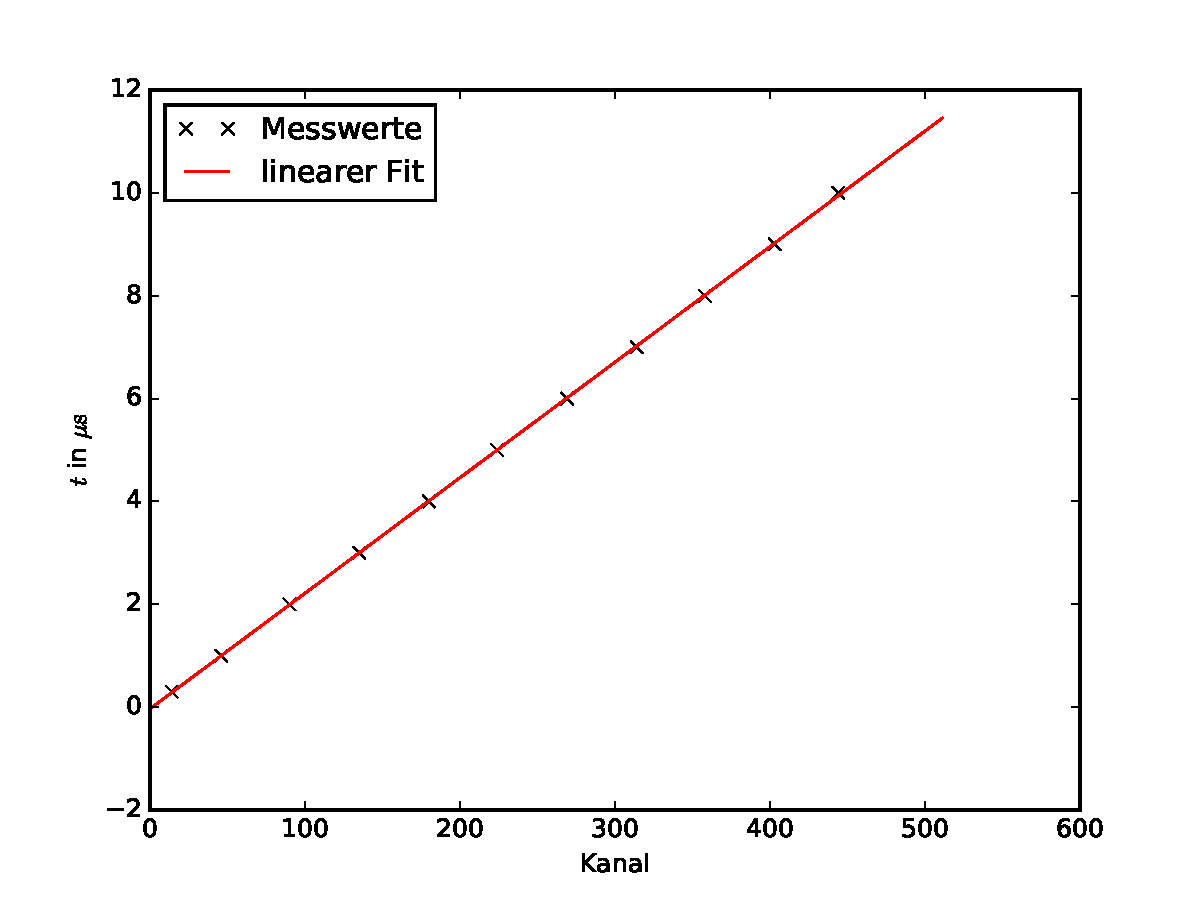
\includegraphics[width = \textwidth]{Pics/Kalibrierung.pdf}
  \caption{Grafische Darstellung der Kanalbelegung und lineare Regression.}
  \label{fig:Kalibrierung}
\end{figure}

\begin{equation}
  T(K) = A\cdot K + B
  \label{eqn:Kalibrierung_Fit}
\end{equation}

Mithilfe von Formel \eqref{eqn:Kalibrierung_Fit} wird eine lineare Regression
durchgeführt, damit ermitteln werden kann, zu welchem Kanal welcher zeitliche Abstand gehört.
Für die Parameter A und B ergeben sich dabei folgende Wert:

\begin{align}
  A &= (0.02247 \pm 0.00005) \,\, \su{\mu s} \\
  B &= (-0.032 \pm 0.014) \,\, \su{\mu s}
\end{align}

\subsection{Bestimmung der Lebensdauer von kosmischen Myonen}

In dem letzten Abschnitt der Auswertung wird die Lebensdauer der Myonen bestimmt.
Die Messung wurde über einen Zeitraum von $T\ua{ges} = 81591$ $\su{s}$ durchgeführt.
Dabei wurden $N\ua{Start} = 1444133$ Startimpulse registriert sowie $N\ua{Stop} =
4255$ Stopimpulse. Die eingestellte Suchzeit beträgt $T\ua{Search} = 10 \, \su{\mu s}$.
Mit diesen Werten lässt sich der Untergrund berechnen. Der Untergrund entsteht aufgrund
der Suchzeit. Sollte innerhalb der Suchzeit ein zweites Myon in den Szintillator
eintreten, kann ein eigentlich nicht auftretender Zerfall von der Apparatur
felhinterpretiert werden. Der Untergrund ergibt sich wie folgt.

\begin{align}
  R &= \frac{N\ua{Start}}{T\ua{ges}} = 17.7 \,\, \frac{\su{Impulse}}{\su{s}}
  \label{eqn:Rate} \\
  N\ua{Search} &= R \cdot T\ua{Search}
  \label{eqn:Nnull}\\
  W(1) &= N\ua{Searcg} \cdot \exp{N\ua{Search}}
  \label{eqn:w1}\\
  U\ua{ges} &= W(1) \cdot N\ua{Start}
  \label{eqn:U1}
\end{align}

Zuerst wird die Rate der pro Sekunde ausgelösten Startsignale bestimmt \eqref{eqn:Rate},
mit der dann die Anzahl von in der Suchzeit ausgelösten Signale \eqref{eqn:Nnull}
bestimmt wird. In der Versuchsanleitung wurde angegeben, dass die Wahrscheinlichkeit,
dass k Myonen in der Suchzeit eintreffen gemäß einer Poisson-Verteilung gegeben ist.
Somit ergibt sich für die Wahrscheinlichkeit, dass ein Myon eintrifft W = 0.00018 $\%$.
Gemäß Formel \eqref{eqn:U1} lässt sich dann die Anzahl der dem Untergrund zuzuordnenden
Signale berechnen. Da sich die Untergrund Signale gleich auf jeden Kanal verteilen,
ergeben sich pro Kanal $U\ua{1} = 0.499$ Signale.

\begin{figure}
  \centering
  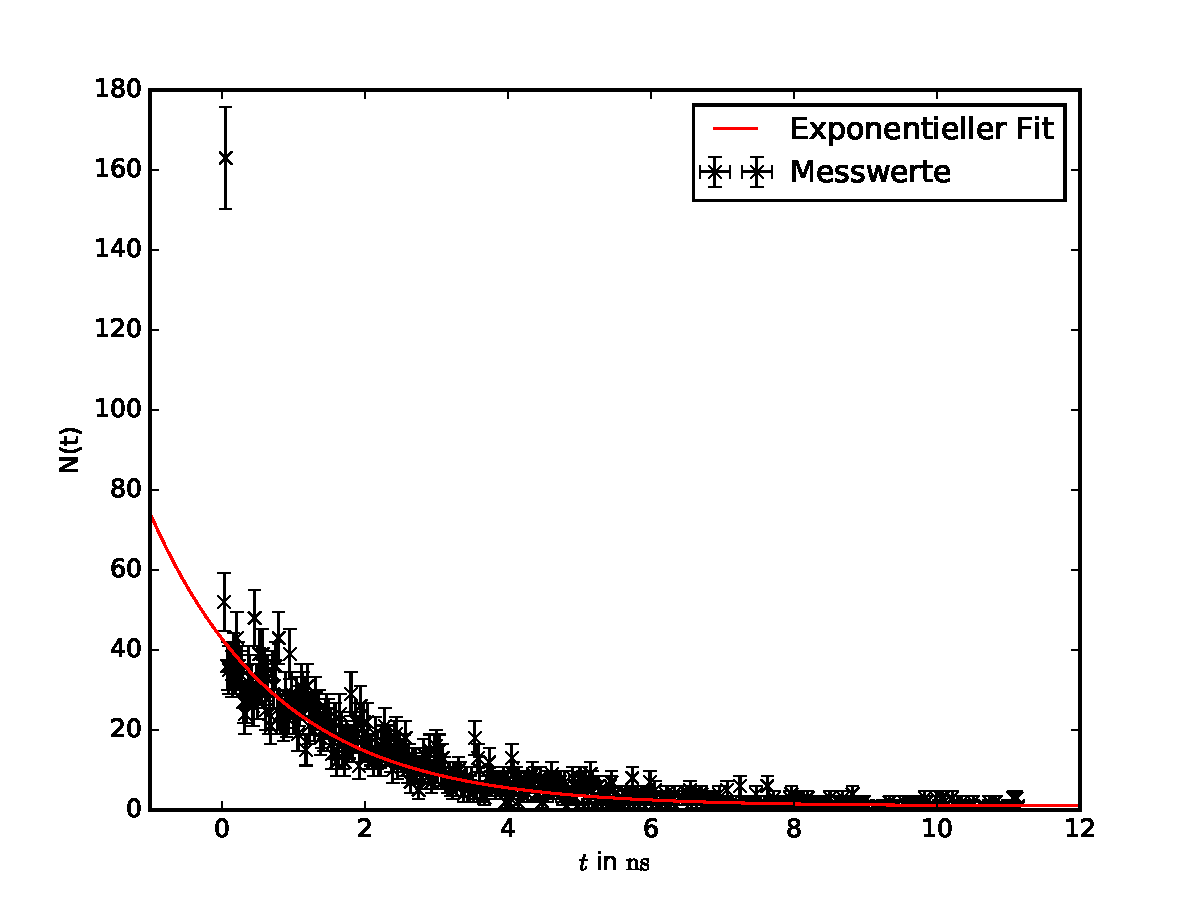
\includegraphics[width = \textwidth]{Pics/Spektrum_gross.pdf}
  \caption{Gemessene Anzahl an Impulsen pro Kanal.}
  \label{fig:Spek_groß}
\end{figure}

Im folgenden wird dieser Wert jedoch nicht verwendet, sondern lediglich mit einem
durch die Regression ermittelten Wert verglichen. Die gemessene Verteilung der
Stopsignale auf die Kanäle ist in Tabelle \ref{tab:Spektrum} dargestellt. Für die
Auswertung wurden
dabei alle Kanäle vernachlässigt, deren gemessener Wert 0 ist. Jedem Kanal mit
der Anzahl $n$ wird als Fehler $\sqrt{n}$ zugeteilt. Da hier ein gewichteter
Fit durchgeführt wird, rufen Werte mit Fehler 0 dabei eine Singularität hervor.

\begin{equation}
  N(t) = N\ua{0} \cdot \exp{-\lambda \cdot t} + U\ua{2}
  \label{eqn:Exponentiell}
\end{equation}

Für die Auswertung der in Abbildung \ref{fig:Spek_groß} dargestellten Werte wird an die Funktion
\eqref{eqn:Exponentiell} gefittet. Für die Parameter ergeben sich zu:

\begin{align}
  N\ua{0} &= (42 \pm 1) \\
  \lambda &= (0.558 \pm 0.018) \cdot 10^{6}\, \frac{1}{\su{s}} \\
  U\ua{2} &= (1.02 \pm 0.13)
\end{align}

Durch die bestimmte Zerfallskonstante $\lambda$ lässt sich dann die mittlere
Lebensdauer $\tau$ der Myonen bestimmen:

\begin{equation}
  \tau = \frac{1}{\lambda} = (1.79 \pm 0.06) \, \su{\mu s}.
\end{equation}

\section{Diskussion}

Die bestimmten Werte sind in Tabelle \ref{tab:ErgebnisseU} und \ref{tab:ErgebnissTau}
zu sehen. In der Auswertung wurde der Untergrund auf zwei verschiedene Arten
bestimmt, wobei der eine ungefähr doppelt so groß ist. Beim Vergleich der bestimmten
Lebensdauer ist ein Abweichung von ca. 18 $\%$ gegenüber dem Literaturwert zu sehen.
Der Literaturwert liegt zudem nicht im Fehlerintervall des bestimmten Wertes.

Für diese Abweichung gibt es mehrere mögliche Ursachen. Einerseits hat sich schon
in der Kalibrierung gezeigt, dass einige Zeiten mehreren Kanälen zugeordnet
werden. Um dieses Fehler zu berücksichtigen hätte auch hier eine Fehlerrechnung
durchgeführt werden müssen, worauf in dieser Auswertung jedoch verzichtet wurde.
Eine weitere Fehlerquelle sind die Anti-Myonen, welche sich mit den Szintillator-Atomen
zu einem angeregten myonischen Atom verbinden und nicht innerhalb der
Suchzeit zerfallen.

\begin{table}
  \centering
  \caption{Ergebnisse für den Untergrund}
  \label{tab:ErgebnisseU}
  \begin{tabular}{c c c c c}
    \toprule
    $U\ua{1}$ & $\increment$ $U\ua{1}$ & $U\ua{2}$ & $\increment$ $U\ua{2}$ & $\frac{U\ua{1}}{U\ua{2}}$ \\
    \midrule
    0.499 & & 1.02 & 0.13 & 0.49 $\pm$ 0.06 \\
    \bottomrule
  \end{tabular}
\end{table}

\begin{table}
  \centering
  \caption{Ergebniss für den Untergrund und Vergleich mit dem Literaturwert. \cite{Taulit}}
  \label{tab:ErgebnissTau}
  \begin{tabular}{c c c c}
    \toprule
    $\tau\ua{\mu,exp}$ & $\tau\ua{\mu,lit}$ & $\frac{\tau\ua{\mu,exp}}{\tau\ua{\mu,lit}}$ \\
    \midrule
    1.79 $\pm$ 0.06 & 2.20 $\pm$ 0 & 0.82 $\pm$ 0.03 \\
    \bottomrule
  \end{tabular}
\end{table}


\section{Messwerte}

\begin{table}
 \centering
 \caption{Gemessene Impulse pro Kanal.}
 \label{tab:Spektrum}
 \begin{tabular}{c|c||c|c||c|c||c|c||c|c||c|c||c|c}
 \toprule
 \multicolumn{2}{c}{1 - 80}    & \multicolumn{2}{c}{81 - 160}  &
 \multicolumn{2}{c}{161 - 240} & \multicolumn{2}{c}{241 - 320} &
 \multicolumn{2}{c}{321 - 400} & \multicolumn{2}{c}{401 - 480} &
 \multicolumn{2}{c}{481 - 512} \\
\cmidrule(lr){1-2}\cmidrule(lr){3-4}\cmidrule(lr){5-6}\cmidrule(lr){7-8}\cmidrule(lr){9-10}\cmidrule(lr){11-12}\cmidrule(lr){13-14}
 K & C & K & C & K & C & K & C & K & C & K & C & K & C \\
 \midrule
 1  & 0   & 81  & 16 & 161 &  5 & 241 &  3 & 321 & 0 & 401 & 0 & 481 & 1\\
 2  & 0   & 82  & 17 & 162 & 13 & 242 &  2 & 322 & 1 & 402 & 2 & 482 & 0\\
 3  & 0   & 83  & 29 & 163 & 10 & 243 &  4 & 323 & 1 & 403 & 1 & 483 & 0\\
 4  & 52  & 84  & 16 & 164 &  5 & 244 &  6 & 324 & 1 & 404 & 1 & 484 & 2\\
 5  & 163 & 85  & 20 & 165 &  4 & 245 &  7 & 325 & 6 & 405 & 0 & 485 & 0\\
 6  & 36  & 86  & 22 & 166 &  3 & 246 &  2 & 326 & 1 & 406 & 0 & 486 & 0\\
 7  & 35  & 87  & 19 & 167 &  6 & 247 &  4 & 327 & 2 & 407 & 0 & 487 & 0\\
 8  & 36  & 88  & 11 & 168 &  8 & 248 &  2 & 328 & 2 & 408 & 1 & 488 & 0\\
 9  & 34  & 89  & 26 & 169 & 12 & 249 &  3 & 329 & 2 & 409 & 0 & 489 & 1\\
 10 & 38  & 90  & 16 & 170 &  7 & 250 &  2 & 330 & 2 & 410 & 0 & 490 & 0\\
 11 & 35  & 91  & 22 & 171 &  8 & 251 &  1 & 331 & 2 & 411 & 1 & 491 & 0\\
 12 & 43  & 92  & 16 & 172 &  7 & 252 &  3 & 332 & 2 & 412 & 1 & 492 & 1\\
 13 & 36  & 93  & 22 & 173 &  5 & 253 &  2 & 333 & 1 & 413 & 0 & 493 & 0\\
 14 & 34  & 94  & 14 & 174 &  6 & 254 &  4 & 334 & 0 & 414 & 1 & 494 & 1\\
 15 & 35  & 95  & 15 & 175 &  7 & 255 &  4 & 335 & 4 & 415 & 1 & 495 & 3\\
 16 & 27  & 96  & 15 & 176 &  7 & 256 &  3 & 336 & 1 & 416 & 0 & 496 & 0\\
 17 & 24  & 97  & 12 & 177 &  7 & 257 &  3 & 337 & 1 & 417 & 1 & 497 & 3\\
 18 & 27  & 98  & 19 & 178 &  8 & 258 &  8 & 338 & 2 & 418 & 2 & 498 & 1\\
 19 & 35  & 99  & 14 & 179 &  2 & 259 &  1 & 339 & 1 & 419 & 0 & 499 & 0\\
 20 & 33  & 100 & 12 & 180 &  7 & 260 &  4 & 340 & 2 & 420 & 1 & 500 & 0\\
 21 & 31  & 101 & 12 & 181 &  5 & 261 &  3 & 341 & 0 & 421 & 0 & 501 & 0\\
 22 & 26  & 102 & 16 & 182 &  3 & 262 &  1 & 342 & 6 & 422 & 1 & 502 & 0\\
 23 & 48  & 103 & 17 & 183 & 13 & 263 &  3 & 343 & 2 & 423 & 0 & 503 & 0\\
 24 & 31  & 104 & 21 & 184 &  9 & 264 &  3 & 344 & 1 & 424 & 0 & 504 & 0\\
 25 & 28  & 105 & 16 & 185 &  8 & 265 &  4 & 345 & 0 & 425 & 0 & 505 & 0\\
 26 & 39  & 106 & 15 & 186 &  8 & 266 &  1 & 346 & 3 & 426 & 0 & 506 & 0\\
 27 & 32  & 107 & 17 & 187 &  2 & 267 &  4 & 347 & 2 & 427 & 2 & 507 & 0\\
 28 & 39  & 108 & 13 & 188 &  6 & 268 &  3 & 348 & 0 & 428 & 0 & 508 & 0\\
 29 & 34  & 109 & 10 & 189 &  5 & 269 &  7 & 349 & 1 & 429 & 1 & 509 & 0\\
 30 & 25  & 110 & 18 & 190 &  4 & 270 &  3 & 350 & 2 & 430 & 0 & 510 & 0\\
 31 & 33  & 111 & 19 & 191 &  7 & 271 &  3 & 351 & 2 & 431 & 2 & 511 & 0\\
 32 & 24  & 112 & 11 & 192 &  7 & 272 &  5 & 352 & 1 & 432 & 1 & 512 & 0\\
 33 & 21  & 113 & 15 & 193 &  4 & 273 &  2 & 353 & 1 & 433 & 1 &     &  \\
 34 & 34  & 114 & 14 & 194 &  7 & 274 &  1 & 354 & 2 & 434 & 1 &     &  \\
 35 & 31  & 115 & 13 & 195 &  7 & 275 &  1 & 355 & 1 & 435 & 0 &     &  \\
 36 & 36  & 116 & 15 & 196 &  9 & 276 &  2 & 356 & 3 & 436 & 2 &     &  \\
 37 & 25  & 117 & 18 & 197 &  8 & 277 &  3 & 357 & 4 & 437 & 2 &     &  \\
 38 & 43  & 118 & 10 & 198 &  4 & 278 &  3 & 358 & 0 & 438 & 1 &     &  \\
 39 & 24  & 119 & 13 & 199 &  4 & 279 &  4 & 359 & 3 & 439 & 1 &     &  \\
 40 & 24  & 120 &  7 & 200 &  4 & 280 &  1 & 360 & 2 & 440 & 3 &     &  \\
 \bottomrule
 \end{tabular}
 \end{table}

\newpage

 \begin{table}
  \centering
  \label{tab:Messwerte2}
  \begin{tabular}{c|c||c|c||c|c||c|c||c|c||c|c||c|c}
  \toprule
  \multicolumn{2}{c}{1 - 80}    & \multicolumn{2}{c}{81 - 160}  &
  \multicolumn{2}{c}{161 - 240} & \multicolumn{2}{c}{241 - 320} &
  \multicolumn{2}{c}{321 - 400} & \multicolumn{2}{c}{401 - 480} &
  \multicolumn{2}{c}{481 - 512} \\
 \cmidrule(lr){1-2}\cmidrule(lr){3-4}\cmidrule(lr){5-6}\cmidrule(lr){7-8}\cmidrule(lr){9-10}\cmidrule(lr){11-12}\cmidrule(lr){13-14}
  K & C & K & C & K & C & K & C & K & C & K & C & K & C \\
  \midrule
 41 & 22  & 121 & 12 & 201 &  8 & 281 &  0 & 361 & 3 & 441 & 2 &     &  \\
 42 & 29  & 122 & 11 & 202 &  2 & 282 &  2 & 362 & 0 & 442 & 1 &     &  \\
 43 & 23  & 123 & 12 & 203 &  5 & 283 &  3 & 363 & 1 & 443 & 1 &     &  \\
 44 & 24  & 124 & 10 & 204 &  7 & 284 &  4 & 364 & 0 & 444 & 0 &     &  \\
 45 & 39  & 125 &  5 & 205 &  4 & 285 &  1 & 365 & 2 & 445 & 0 &     &  \\
 46 & 29  & 126 & 10 & 206 &  7 & 286 &  0 & 366 & 0 & 446 & 1 &     &  \\
 47 & 24  & 127 &  8 & 207 &  5 & 287 &  3 & 367 & 3 & 447 & 3 &     &  \\
 48 & 24  & 128 & 14 & 208 &  9 & 288 &  0 & 368 & 1 & 448 & 0 &     &  \\
 49 & 28  & 129 & 12 & 209 &  5 & 289 &  3 & 369 & 1 & 449 & 1 &     &  \\
 50 & 19  & 130 & 11 & 210 &  7 & 290 &  3 & 370 & 2 & 450 & 3 &     &  \\
 51 & 26  & 131 & 10 & 211 &  7 & 291 &  0 & 371 & 0 & 451 & 3 &     &  \\
 52 & 31  & 132 & 15 & 212 &  6 & 292 &  4 & 372 & 0 & 452 & 2 &     &  \\
 53 & 29  & 133 &  7 & 213 &  7 & 293 &  4 & 373 & 2 & 453 & 1 &     &  \\
 54 & 28  & 134 &  8 & 214 &  4 & 294 &  5 & 374 & 2 & 454 & 0 &     &  \\
 55 & 15  & 135 & 15 & 215 &  3 & 295 &  2 & 375 & 2 & 455 & 0 &     &  \\
 56 & 31  & 136 & 16 & 216 &  7 & 296 &  3 & 376 & 2 & 456 & 0 &     &  \\
 57 & 21  & 137 & 10 & 217 &  1 & 297 &  3 & 377 & 2 & 457 & 3 &     &  \\
 58 & 24  & 138 & 15 & 218 &  3 & 298 &  3 & 378 & 2 & 458 & 2 &     &  \\
 59 & 24  & 139 &  9 & 219 &  4 & 299 &  0 & 379 & 2 & 459 & 0 &     &  \\
 60 & 22  & 140 & 13 & 220 &  3 & 300 &  4 & 380 & 0 & 460 & 0 &     &  \\
 61 & 28  & 141 & 10 & 221 &  8 & 301 &  4 & 381 & 3 & 461 & 1 &     &  \\
 62 & 25  & 142 &  8 & 222 &  6 & 302 &  3 & 382 & 1 & 462 & 0 &     &  \\
 63 & 25  & 143 &  7 & 223 &  3 & 303 &  3 & 383 & 0 & 463 & 2 &     &  \\
 64 & 18  & 144 &  9 & 224 &  1 & 304 &  2 & 384 & 1 & 464 & 1 &     &  \\
 65 & 20  & 145 &  6 & 225 &  8 & 305 &  1 & 385 & 1 & 465 & 0 &     &  \\
 66 & 19  & 146 &  5 & 226 &  8 & 306 &  2 & 386 & 2 & 466 & 1 &     &  \\
 67 & 23  & 147 &  8 & 227 &  7 & 307 &  3 & 387 & 2 & 467 & 0 &     &  \\
 68 & 24  & 148 &  9 & 228 &  1 & 308 &  2 & 388 & 0 & 468 & 1 &     &  \\
 69 & 23  & 149 &  8 & 229 &  7 & 309 &  3 & 389 & 3 & 469 & 0 &     &  \\
 70 & 21  & 150 & 10 & 230 &  5 & 310 &  2 & 390 & 1 & 470 & 2 &     &  \\
 71 & 14  & 151 &  9 & 231 &  2 & 311 &  2 & 391 & 0 & 471 & 0 &     &  \\
 72 & 17  & 152 &  6 & 232 &  9 & 312 &  4 & 392 & 2 & 472 & 0 &     &  \\
 73 & 22  & 153 &  4 & 233 &  7 & 313 &  1 & 393 & 0 & 473 & 0 &     &  \\
 74 & 12  & 154 &  8 & 234 &  6 & 314 &  1 & 394 & 1 & 474 & 0 &     &  \\
 75 & 14  & 155 &  8 & 235 &  1 & 315 &  1 & 395 & 4 & 475 & 0 &     &  \\
 76 & 24  & 156 &  6 & 236 &  2 & 316 &  2 & 396 & 2 & 476 & 1 &     &  \\
 77 & 20  & 157 &  6 & 237 &  6 & 317 &  5 & 397 & 0 & 477 & 1 &     &  \\
 78 & 14  & 158 &  8 & 238 &  5 & 318 &  0 & 398 & 2 & 478 & 0 &     &  \\
 79 & 12  & 159 &  4 & 239 &  2 & 319 &  0 & 399 & 0 & 479 & 0 &     &  \\
 80 & 18  & 160 & 18 & 240 &  4 & 320 &  2 & 400 & 2 & 480 & 2 &     &  \\
 \bottomrule
 \end{tabular}
 \end{table}

